\subsection{Charm baryons}

In this section we summarize the present status of excited charm
baryons, decaying strongly or electromagnetically. We list their
masses (or the mass difference between the excited baryon and the
corresponding ground state), natural widths, decay modes, and 
assigned quantum numbers. 
Table~\ref{sumtable1} summarizes the excited $\Lambda_c^+$ baryons.  
The first two states, $\Lambda_c(2595)^+$ and $\Lambda_c(2625)^+$,
are well-established. 
Based on the measured masses, it is believed they are orbitally 
excited $\Lambda_c^+$ baryons with total angular momentum of the
light quarks $L=1$. Thus their quantum numbers are assigned to be 
$J^P=(\frac{1}{2})^-$ and $J^P=(\frac{3}{2})^-$, respectively. 
Recently, their masses 
%and widths 
were precisely measured by CDF~\cite{Aaltonen:2011sf}: 
$M(\Lambda_c(2595)^+)=2592.25\pm 0.24\pm 0.14$~MeV/c$^2$ and
$M(\Lambda_c(2625)^+)=2628.11\pm 0.13\pm 0.14$~MeV/c$^2$. 

The next two states, $\Lambda_c(2765)^+$ and $\Lambda_c(2880)^+$, 
were discovered by CLEO~\cite{Artuso:2000xy} in the $\Lambda_c^+\pi^+\pi^-$ 
final state. CLEO found that $\Lambda_c(2880)^+$ decays also through
the $\Sigma_c(2445)^{++/0}\pi^{-/+}$ mode. 
Later, \babar~\cite{Aubert:2006sp} 
observed that this state has also a $D^0 p$ decay mode. It is the 
first example of an excited charm baryon decaying into a charm meson 
and a light baryon. (Excited charm baryons typically decay into charm 
baryons and light mesons.) In that analysis, \babar observed for the
first time an additional state, $\Lambda_c(2940)^+$, 
which decays into $D^0 p$. Looking for the $D^+ p$ final state,
\babar found no signal; this implies that the $\Lambda_c(2880)^+$ 
and $\Lambda_c(2940)^+$ are really $\Lambda_c^+$ excited states
rather than $\Sigma_c$ excitations. 
Belle reported the result of an angular analysis that favors
$5/2$ for the $\Lambda_c(2880)^+$ spin hypothesis. 
Moreover, the measured ratio of branching fractions 
${\cal B}(\Lambda_c(2880)^+\rightarrow \Sigma_c(2520)\pi^{\pm})/{\cal B}(\Lambda_c(2880)^+\rightarrow \Sigma_c(2455)\pi^{\pm})=(0.225\pm 0.062\pm 0.025)$, combined 
with theoretical predictions based on HQS~\cite{Isgur:1991wq,Cheng:2006dk}, 
favor even parity.     
The current open questions in the excited $\Lambda_c^+$ family are
the determination of quantum numbers for almost all states, and 
the nature of the $\Lambda_c(2765)^+$ state, \ie\ whether it is
an excited $\Sigma_c^+$ or $\Lambda_c^+$.

%\begin{sidewaystable}
\begin{table}[t]
\caption{Summary of excited $\Lambda_c^+$ baryons family.} 
\vskip0.15in
\resizebox{0.99\textwidth}{!}{
\begin{tabular}{c|c|c|c|c}
\hline
Charmed Baryon   & Mode  & Mass & Natural Width  & $J^P$  \\
Excited State &  &  (MeV/c$^2$) & (MeV/c$^2$)  \\
\hline
$\Lambda_c(2595)^+$ & $\Lambda_c^+\pi^+\pi^-$, $\Sigma_c\pi$ &  $2595.4\pm 0.6$ & $3.6^{+2.0}_{-1.3}$  & $1/2^-$  \\
\hline
$\Lambda_c(2625)^+$ & $\Lambda_c^+\pi^+\pi^-$, $\Sigma_c\pi$ & $2628.1\pm 0.6$ & $<1.9$ & $3/2^-$  \\
\hline
$\Lambda_c(2765)^+$ & $\Lambda_c^+\pi^+\pi^-$, $\Sigma_c\pi$ & $2766.6\pm 2.4$ & $50$ & ??  \\
\hline
$\Lambda_c(2880)^+$ & $\Lambda_c^+\pi^+\pi^-$, $\Sigma_c\pi$,  &$2881.53\pm 0.35$ & $5.8\pm 1.1$ & $5/2^+$ \\
 &  $\Sigma_c(2520)\pi$, $D^0p$     & & & (experimental evidence) \\
\hline
$\Lambda_c(2940)^+$ & $D^0p$, $\Sigma_c\pi$ & $2939.3^{+1.4}_{-1.5}$ & $17^{+8}_{-6}$  & ??  \\
\hline 
\end{tabular}
}
\label{sumtable1} 
\end{table}
%\end{landscape}
%\end{sidewaystable}


Table~\ref{sumtable2} summarizes the excited $\Sigma_c^{++,+,0}$ baryons.
The triplet of $\Sigma_c(2520)^{++,+,0}$ baryons is well-established. 
Recently Belle~\cite{SHLee:2014} 
%%%%%%%%%%%%% CDF~\cite{Aaltonen:2011sf}
precisely measured the mass differences (see above for the definition)  
and widths of the double charged and neutral members of this triplet.
The results are
\begin{eqnarray}
\Delta M(\Sigma_c(2520)^{++}) & = & (231.99\pm 0.10\pm 0.02){\rm\ MeV}/c^2 \\ 
\Gamma(\Sigma_c(2520)^{++}) & = & (14.77\pm 0.25^{+0.18}_{-0.30}){\rm\ MeV} \\ 
\Delta M(\Sigma_c(2520)^{0}) & = & (231.98\pm 0.11\pm 0.04){\rm\ MeV}/c^2 \\ 
\Gamma(\Sigma_c(2520)^{0}) & = & (15.41\pm 0.41^{+0.20}_{-0.32}){\rm\ MeV}\,.
\end{eqnarray} 
%\Delta M(\Sigma_c(2520)^{++})& =& (231.99\pm 0.10\pm 0.02)$~MeV/c$^2$, 
%$\Gamma(\Sigma_c(2520)^{++})=(14.77\pm 0.25^{+0.18}_{-0.30})$~MeV/c$^2$ and 
%$\Delta M(\Sigma_c(2520)^{0})=(231.98\pm 0.11\pm 0.04)$~MeV/c$^2$, 
%$\Gamma(\Sigma_c(2520)^{0})=(15.41\pm 0.41^{+0.20}_{-0.32})$~MeV/c$^2$, respectively. 
This short list of excited $\Sigma_c$ baryons completes the triplet 
of $\Sigma_c(2800)$ states observed by Belle~\cite{Mizuk:2004yu}. Based 
on the measured masses and theoretical predictions~\cite{Copley:1979wj,Pirjol:1997nh}, 
these states are identified as members of the predicted $\Sigma_{c2}$ $3/2^-$
triplet. From a study of resonant substructure 
in $B^-\rightarrow \Lambda_c^+\bar{p}\pi^-$ decays, \babar found 
a significant signal for $\Lambda_c^+\pi^-$ with a mean value 
higher than that measured by Belle by about $3\sigma$
(Table~\ref{sumtable2}). The decay widths measured by
Belle and \babar are consistent.


%\begin{sidewaystable}
\begin{table}[!htb]
\caption{Summary of excited $\Sigma_c^{++,+,0}$ baryons family.} 
\vskip0.15in
\resizebox{\textwidth}{!}{
 \begin{tabular}{c|c|c|c|c}
\hline
Charmed Baryon   & Mode  & $\Delta M$ & Natural Width  & $J^P$  \\
Excited State &  &  (MeV/c$^2$) & (MeV/c$^2$)  \\
\hline
$\Sigma_c(2520)^{++}$ &$\Lambda_c^+\pi^+$  & $231.99\pm 0.10\pm 0.02$ & $14.77\pm 0.25^{+0.18}_{-0.30}$ & $3/2^+$   \\
$\Sigma_c(2520)^{+}$ &$\Lambda_c^+\pi^+$  & $231.0\pm 2.3$ & $<17$~@~90$\%$~CL & $3/2^+$ \\
$\Sigma_c(2520)^{0}$ &$\Lambda_c^+\pi^+$  & $231.98\pm 0.11\pm 0.04$ & $15.41\pm 0.41^{+0.20}_{-0.32}$ & $3/2^+$    \\
\hline
$\Sigma_c(2800)^{++}$ & $\Lambda_c^+\pi^{+}$ & $514.5^{+3.4+2.8}_{-3.1-4.9}$ & $75^{+18+12}_{-13-11}$ & tentatively identified      \\
$\Sigma_c(2800)^{+}$ & $\Lambda_c^+\pi^{0}$&$505.4^{+5.8+12.4}_{-4.6-2.0}$ &$62^{+37+52}_{-23-38}$ & as members of the predicted  \\
$\Sigma_c(2800)^{0}$ & $\Lambda_c^+\pi^{-}$&$515.4^{+3.2+2.1}_{-3.1-6.0}$ & $61^{+18+22}_{-13-13}$ &$\Sigma_{c2}$ $3/2^-$ isospin triplet  \\
 & $\Lambda_c^+\pi^{-}$ & $560\pm 8\pm 10$ & $86^{+33}_{-22}$  \\


\hline 
\end{tabular}
}
\label{sumtable2} 
\end{table}
%\end{landscape}
%\end{sidewaystable}
% =====================================================================================

Table~\ref{sumtable3} summarizes the excited $\Xi_c^{+,0}$ and $\Omega_c^0$ 
baryons. Recently, the list of excited $\Xi_c$ baryons has increased,
with several states having masses above 2900~MeV/c$^2$ and decaying into 
$\Lambda_c^+ K^-$, $\Lambda_c^+ K^{-/0}\pi^{+/-}$ and $\Sigma_c(2455/2520) K$. 
Some of these states ($\Xi_c(2980)^+$ and $\Xi_c(3080)^{+,0}$) are seen by
both Belle~\cite{Chistov:2006zj,YKato:2014} 
and \babar~\cite{Aubert:2007dt} and are considered well-established.
%All others need to be confirmed or studied in more depth. 
The $\Xi_c(2930)^0$ state decaying into $\Lambda_c^+ K^-$ is seen
by \babar~\cite{Aubert:2007eb} but still needs confirmation.  
The $\Xi_c(3055)^+$ found in the $\Sigma_c(2455)^{++}\pi^-$ final
state by \babar~\cite{Aubert:2007dt} was recently confirmed by
Belle~\cite{YKato:2014}. 
The width and mass measurements for the $\Xi_c(3055)^+$
listed in Table~\ref{sumtable3} 
 are not averaged but quoted separately for \babar and Belle. 
However, the $\Xi_c(3123)^+$ observed by \babar~\cite{Aubert:2007dt}
in the $\Sigma_c(2520)^{++}\pi^-$ final state has not been
confirmed by Belle~\cite{YKato:2014} with twice as much statistics.   
We note that Belle~\cite{YKato:2014} recently performed the first
significant measurement of the $\Xi_c(2645)^+$ width, as listed
in Table~\ref{sumtable3}. 


The excited $\Omega_c^0$ double charm baryon is seen by both 
\babar~\cite{Aubert:2006je} and Belle~\cite{Solovieva:2008fw};
the mass differences $\delta M=M(\Omega_c^{*0})-M(\Omega_c^0)$ 
measured by the experiments are in good agreement
and are also consistent with most theoretical 
predictions~\cite{Rosner:1995yu,Glozman:1995xy,Jenkins:1996de,
Burakovsky:1997vm}. 
   

%\begin{sidewaystable}
\begin{table}[b]
\caption{Summary of excited $\Xi_c^{+,0}$ and $\Omega_c^0$ baryons families.} 
\vskip0.15in
\resizebox{\textwidth}{!}{
\begin{tabular}{c|c|c|c|c}
\hline
Charmed Baryon   & Mode  & Mass & Natural Width  & $J^P$  \\
Excited State &  &  (MeV/c$^2$) & (MeV/c$^2$)  \\
\hline
$\Xi_c'^+$ & $\Xi_c^+\gamma$ & $2575.6\pm 3.1$  &  & $1/2^+$    \\
$\Xi_c'^0$ & $\Xi_c^0\gamma$ & $2577.9\pm 2.9$  &  & $1/2^+$   \\
\hline
$\Xi_c(2645)^+$ & $\Xi_c^0\pi^+$ & $2645.9^{+0.6}_{-0.5}$  & $2.6\pm 0.2\pm 0.4$ & $3/2^+$   \\
$\Xi_c(2645)^0$ & $\Xi_c^+\pi^-$ & $2645.9\pm 0.5$  & $<5.5$ & $3/2^+$   \\
\hline
$\Xi_c(2790)^+$ &$\Xi_c'^0\pi^+$ & $2789.1\pm 3.2$ & $<15$ & $1/2^-$   \\
$\Xi_c(2790)^0$ &$\Xi_c'^+\pi^-$ & $2791.8\pm 3.3$ & $<12$ & $1/2^-$   \\
\hline
$\Xi_c(2815)^+$ &$\Xi_c^+\pi^+\pi^-$, $\Xi_c(2645)^0\pi^+$ & $2816.6\pm 0.9$ & $<3.5$ &  $3/2^-$  \\
$\Xi_c(2815)^0$ & $\Xi_c^0\pi^+\pi^-$, $\Xi_c(2645)^+\pi^-$& $2819.6\pm 1.2$  & $<6.5$  & $3/2^-$   \\
\hline
$\Xi_c(2930)^0$ & $\Lambda_c^+ K^-$ & $2931.6\pm 6$ & $36\pm 13$ & ??     \\
\hline
$\Xi_c(2980)^+$ & $\Lambda_c^+K^-\pi^+$, $\Sigma_c^{++}K^-$, $\Xi_c(2645)^0\pi^+$
%\footnote{this mode obs. by Belle~\cite{lesiak} but natural width is systematically lower than in other modes }
 &  $2971.4\pm 3.3$  & $26\pm 7$ & ??     \\
$\Xi_c(2980)^0$ & $\Xi_c(2645)^+\pi^-$
%\footnote{this mode obs. by Belle~\cite{lesiak} (6.1$\sigma$) but natural width is systematically lower than in other modes } 
&  $2968.0\pm 2.6$ &$20\pm 7$ & ??       \\
\hline
$\Xi_c(3055)^+$ & $\Sigma_c^{++}K^-$ & 	$3054.2\pm 1.3$ (\babar) &     	$17\pm 13$ (\babar) & ??   \\
       &        &   $3058.1\pm 1.0\pm 2.1$   (Belle)   &   $9.7\pm 3.4\pm 3.3$  (Belle)           \\
%$\Xi_c(3055)^0$ & &  & & ??    \\
\hline
$\Xi_c(3080)^+$ & $\Lambda_c^+K^-\pi^+$, $\Sigma_c^{++}K^-$, $\Sigma_c(2520)^{++}K^-$ & $3077.0\pm 0.4$ & $5.8\pm 1.0$ & ??   \\
$\Xi_c(3080)^0$ &$\Lambda_c^+ K^0_S\pi^-$, $\Sigma_c^0K^0_S$, $\Sigma_c(2520)^{0}K^0_S$ & $3079.9\pm 1.4$ & $5.6\pm 2.2$ & ??   \\
\hline
%$\Xi_c(3123)^+$ &$\Sigma_c(2520)^{++}K^-$ & $3122.9\pm 1.3$ & $4\pm 4$ & ??   \\
%\hline
\\
\hline
$\Omega_c(2770)^0$ & $\Omega_c^0\gamma$& $2765.9\pm 2.0$  & $70.7^{+0.8}_{-0.9}$ & $3/2^+$  \\
\hline 
\end{tabular}
}
\label{sumtable3} 
\end{table}
%\end{landscape}
%\end{sidewaystable}
 

Figure~\ref{charm:leveldiagram} shows the levels of excited charm
baryons along with corresponding transitions between them, and
also transitions to the ground states.
\begin{figure}[!htb]
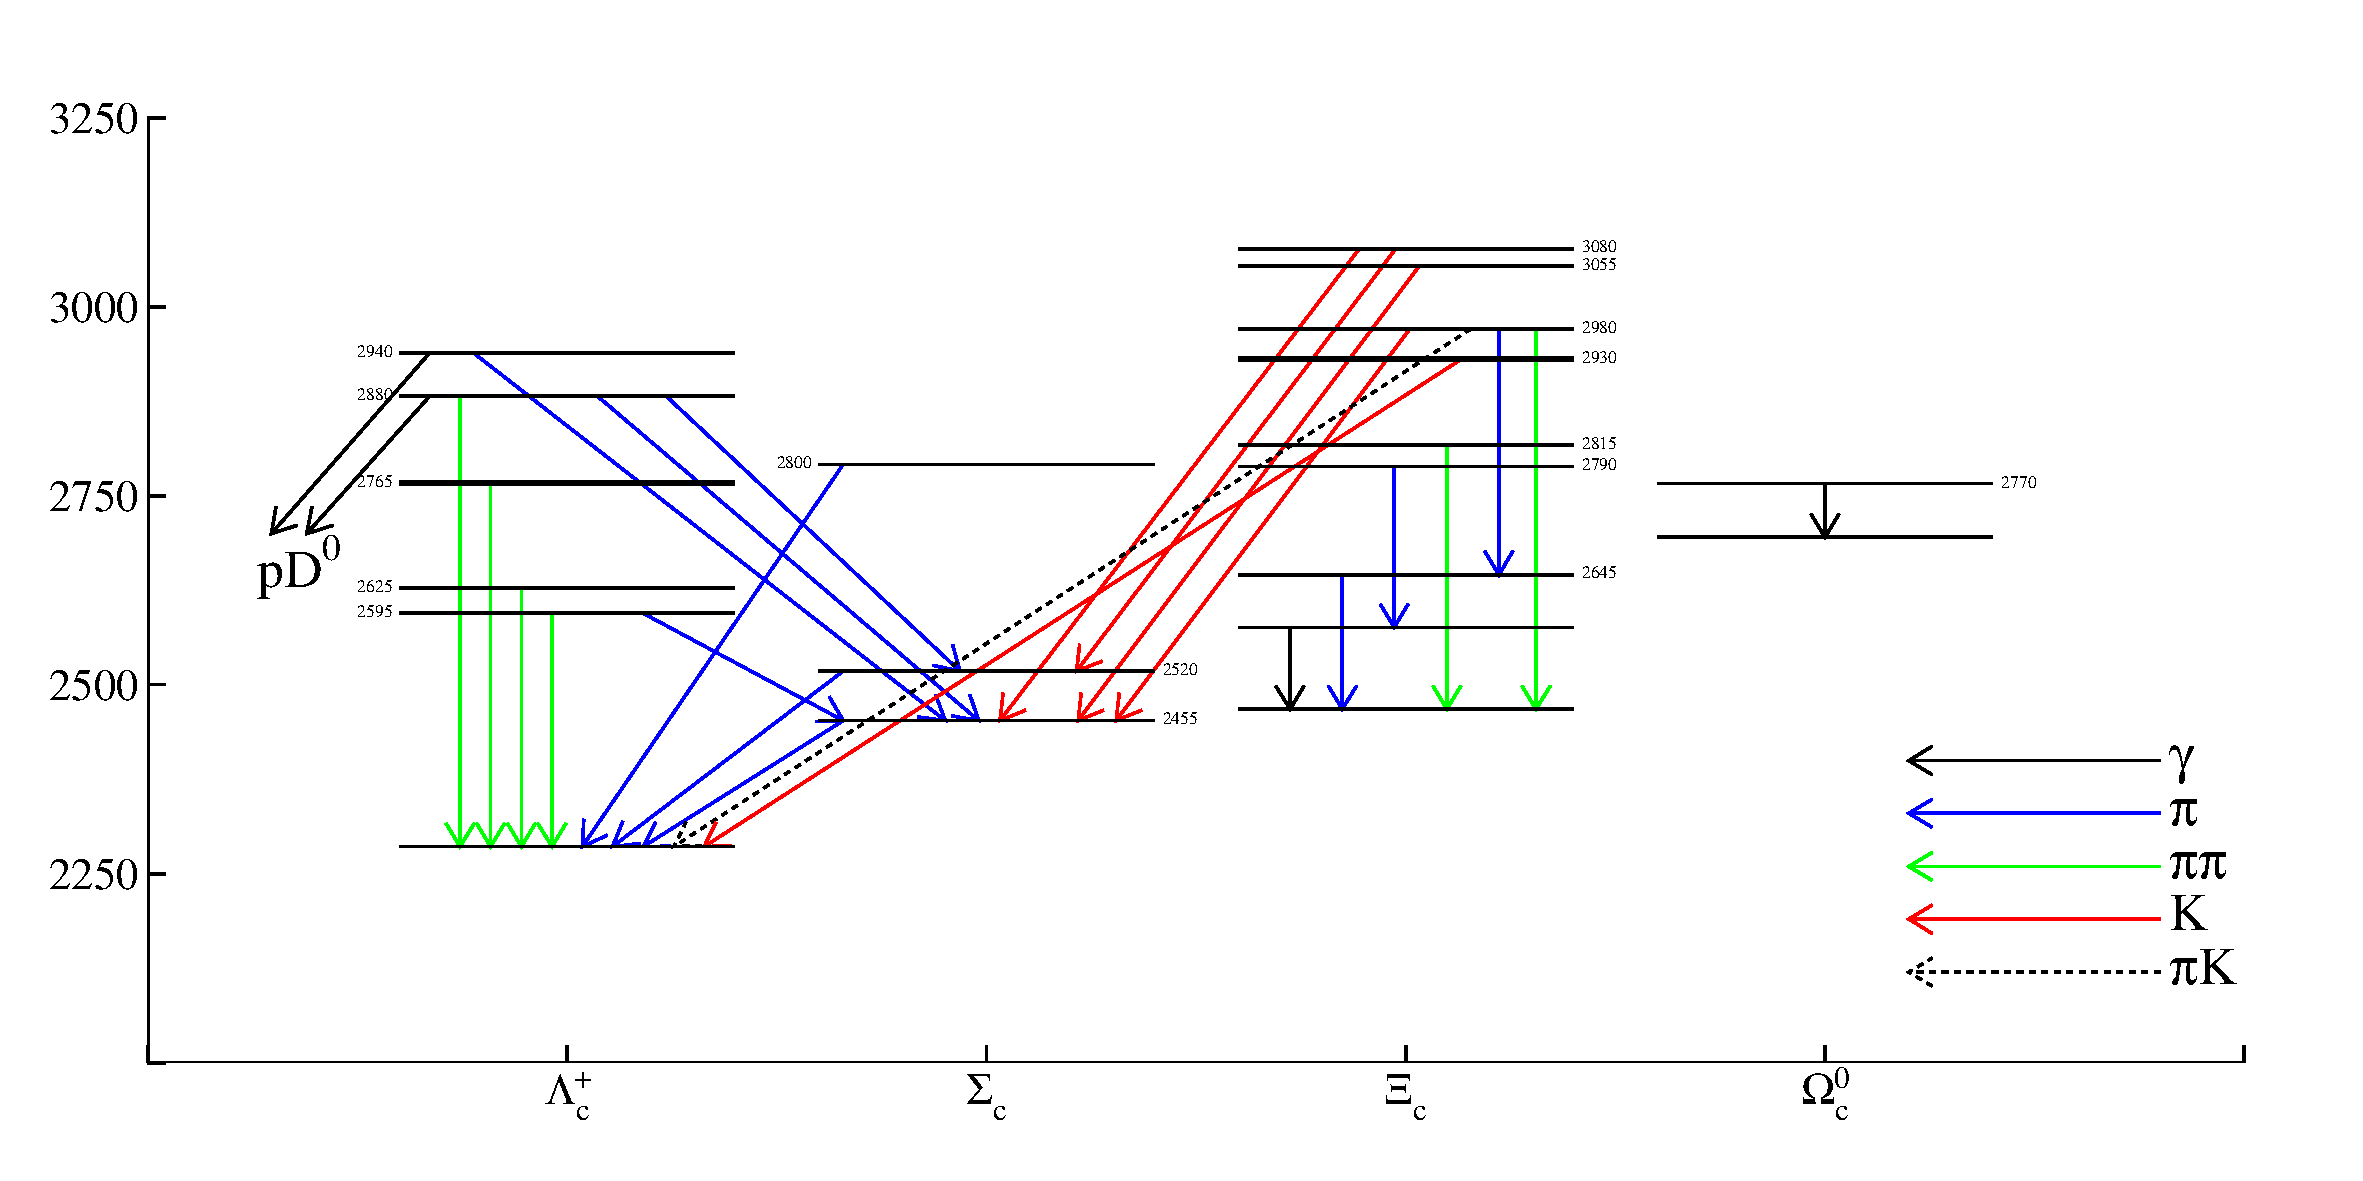
\includegraphics[width=1.0\textwidth]{./figures/charm/charm_baryons2014.pdf}
\caption{Level diagram for excited charm baryons.}
\label{charm:leveldiagram}
\end{figure} 
In summary, we note that Belle and \babar  recently discovered
that transitions between families are possible, \ie\ between the 
$\Xi_c$ and $\Lambda_c^+$ families of excited charm baryons. Also,
highly excited $\Lambda_c^+$ baryons are found to decay into 
a charm meson and a proton.    



